\documentclass[tikz]{standalone}
\usepackage{pgfplots}
\pgfplotsset{compat=1.15}
\usepackage{mathrsfs}
\usetikzlibrary{arrows,calc}
\usepackage{tkz-euclide}
\pagestyle{empty}

\definecolor{AngleClr}{rgb}{0,0.39215686274509803,0}
\definecolor{ShapeClr}{rgb}{0.6,0.2,0}
\definecolor{BlueSqr}{RGB}{5,81,163}
\definecolor{RedSqr}{RGB}{0, 156, 0}

\begin{document}

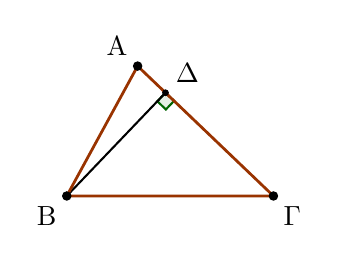
\begin{tikzpicture}[scale=.75]
\tkzSetUpLine[line width=1pt,color=black]
\tkzSetUpPoint[fill=black]

\tkzDefPoints{0/0/B,3.5/0/C,1.2/2.2/A}
\tkzDefPointBy[projection=onto A--C](B)\tkzGetPoint{D}

\tkzFillPolygon[fill=white](A,B,C)

\tkzMarkRightAngle[line width=0.75pt, size=.2,color=AngleClr,fill=AngleClr,fill opacity=0.1](B,D,C)
\tkzDrawSegment[line width=0.75pt,color=black](B,D)

\tkzDrawPolygon[color=ShapeClr](A,B,C)



\tkzDrawPoints[size=3](A,B,C)
\tkzDrawPoints[size=2](D)
\tkzLabelPoint[above left](A){$\rm A$}
\tkzLabelPoint[above right](D){$\rm \Delta$}
\tkzLabelPoint[below left](B){$\rm B$}
\tkzLabelPoint[below right](C){$\rm \Gamma$}


\end{tikzpicture}

\end{document}
